%!TEX root = ../documentation.tex
\chapter{Datenvorverarbeitung}
\label{ch:data_preprocessing}

\section{Bilddaten}

In der vorherigen Datenanalyse wurden folgende Probleme herausgestellt:

\begin{enumerate}
	\item{Dimensionsunterschiede}
	\item{Farbunterschiede}
	\item{Kontrastunterschiede}
\end{enumerate}

Diese sollen nun mit geeigneten Vorverarbeitungsschritten gelöst werden.

Die Bilder müssen als Eingabe für das Model in einer einheitlichen Größe vorliegen. Dazu skalieren wir alle Bilder auf den Schwerpunkt der Dimensionen, welcher bei 320 x 320 Pixeln liegt.
Nur drei der Bilder sind kleiner als 320 x 320 Pixel und mussen damit vergrößert werden um die gewünschte Dimension zu erreichen. Bei einer Vergrößerung können Artifakte im Bild auftreten, welche das Model beeinflussen können. Aufgrund der geringen Anzahl können diese in unserem Fall vernachlässigt werden.\\
Farbliche Informationen spielen in den Röntgenbildern keine Rolle. Daher verwerfen wir die Farbinformationen und wandeln alle Farbbilder in Schwarzweißbilder um.\\
Weiterhin werden die Kontrastunterschiede über einen Histogrammausgleich verringert. Dadurch werden die Bilder, welche aus vielen verschiedenen Quellen stammen, homogenisiert.

\begin{figure}[H]
	\centering
	\begin{subfigure}[b]{0.45\textwidth}
		\centering
		\includegraphics[width=0.5\textwidth]{../images/42081.jpg}
		\caption{Originalbild 42081.jpg\\1524 x 1516 Pixel}
	\end{subfigure} \hfill
	\begin{subfigure}[b]{0.45\textwidth}
		\centering
		\includegraphics[width=0.5\textwidth]{../train_data/42081.jpg}
		\caption{Vorverarbeitetes Bild\\320 x 320 Pixel}
	\end{subfigure} \hfill
	\caption{Vergleich eines Originalbildes mit dem daraus resultierenden vorverarbeiten Bild}
\end{figure}

\section{Datenaugmentation}

Bezüglich der Klassen haben wir in der zweiten Konstellation (zusammengefasste Krankheiten) eine ungleiche Verteilung festgestellt. Wie in \cite{BUDA2018249} herausgestellt wird, beeinflusst dies die Leistung des Models in negativer Weise.\\
Um dieses Problem zu umgehen führen wir eine Offline-Datenaugmentation ähnlich wie in \cite{UCAR2020109761} beschrieben durch. Dabei werden aus einem Quellbild durch Transformationen mehrere zusätzliche Bilder erstellt. Diese werden dann in einem Verzeichnis auf der Festplatte abgelegt (offline).

Dazu haben wir zunächst die folgenden Basistransformationen bereitgestellt.
\begin{enumerate}
	\item{Vertikale Spiegelung (Flip)}
	\item{Aufhellen (Bright)}
	\item{Verdunkeln (Dark)}
	\item{Gaußsche Unschärfe (Noise)}
	\item{Scherung (Shear)}
	\item{Rotation (Rotation)}
\end{enumerate}
Um die Anzahl der Transformationen weiter zu erhöhen und damit möglichst viele unterschiedliche Bilder zu erzeugen, haben wir weiterhin Kombinationen der Basistransformationen definiert.
Insgesamt erreichen wir somit 20 Transformationen. Diese werden in Abbildung \ref{fig:augmentation} auf Seite \pageref{fig:augmentation} anhand eines Beispiels visualisiert.

Durch die Datenaugmentation kann das Ungleichgewicht bei der Verteilung der Klassen komplett aufgehoben werden, wie von der Abbildung \ref{fig:balancing} auf Seite \pageref{fig:balancing} dargestellt wird.
In der ersten Konstellation kann die Anzahl der COVID-19 Bilder deutlich erhöht werden, welches zu einer besseren Erkennung der Krankheit führen sollte.

\begin{figure}[H]
	\centering
	\begin{subfigure}[b]{0.2\textwidth}
		\includegraphics[width=\textwidth]{../train_data/18121.png}
		\caption{Vorverarbeitetes Bild}
	\end{subfigure} \hfill
	\begin{subfigure}[b]{0.2\textwidth}
		\includegraphics[width=\textwidth]{../aug_data/Augbright_18121.png}
		\caption{Bright}
	\end{subfigure} \hfill
	\begin{subfigure}[b]{0.2\textwidth}
		\includegraphics[width=\textwidth]{../aug_data/Augdark_18121.png}
		\caption{Dark}
	\end{subfigure} \hfill
	\begin{subfigure}[b]{0.2\textwidth}
		\includegraphics[width=\textwidth]{../aug_data/Augnoise_18121.png}
		\caption{Noise}
	\end{subfigure} \hfill
	\begin{subfigure}[b]{0.2\textwidth}
		\includegraphics[width=\textwidth]{../aug_data/Augflip_18121.png}
		\caption{Flip}
	\end{subfigure} \hfill
	\begin{subfigure}[b]{0.2\textwidth}
		\includegraphics[width=\textwidth]{../aug_data/Augrotation_18121.png}
		\caption{Rotation}
	\end{subfigure} \hfill
	\begin{subfigure}[b]{0.2\textwidth}
		\includegraphics[width=\textwidth]{../aug_data/Augshear_18121.png}
		\caption{Shear}
	\end{subfigure} \hfill
	\begin{subfigure}[b]{0.2\textwidth}
		\includegraphics[width=\textwidth]{../aug_data/Augflip_dark_18121.png}
		\caption{Flip + Dark}
	\end{subfigure} \hfill
	\begin{subfigure}[b]{0.2\textwidth}
		\includegraphics[width=\textwidth]{../aug_data/Augflip_dark_noise_18121.png}
		\caption{Flip + Dark + Noise}
	\end{subfigure} \hfill
	\begin{subfigure}[b]{0.2\textwidth}
		\includegraphics[width=\textwidth]{../aug_data/Augflip_rotation_18121.png}
		\caption{Flip + Rotation}
	\end{subfigure} \hfill
	\begin{subfigure}[b]{0.2\textwidth}
		\includegraphics[width=\textwidth]{../aug_data/Augflip_rotation_bright_shear_18121.png}
		\caption{Flip + Rotation + Bright + Shear}
	\end{subfigure} \hfill
	\begin{subfigure}[b]{0.2\textwidth}
		\includegraphics[width=\textwidth]{../aug_data/Augflip_shear_18121.png}
		\caption{Flip + Shear}
	\end{subfigure} \hfill
	\begin{subfigure}[b]{0.2\textwidth}
		\includegraphics[width=\textwidth]{../aug_data/Augflip_shear_noise_18121.png}
		\caption{Flip + Shear + Noise}
	\end{subfigure} \hfill
	\begin{subfigure}[b]{0.2\textwidth}
		\includegraphics[width=\textwidth]{../aug_data/Augflip_shear_rotation_18121.png}
		\caption{Flip + Shear + Rotation}
	\end{subfigure} \hfill
	\begin{subfigure}[b]{0.2\textwidth}
		\includegraphics[width=\textwidth]{../aug_data/Augnoise_bright_shear_18121.png}
		\caption{Noise + Bright + Shear}
	\end{subfigure} \hfill
	\begin{subfigure}[b]{0.2\textwidth}
		\includegraphics[width=\textwidth]{../aug_data/Augnoise_rotation_18121.png}
		\caption{Noise + Rotation}
	\end{subfigure} \hfill
	\begin{subfigure}[b]{0.2\textwidth}
		\includegraphics[width=\textwidth]{../aug_data/Augrotation_bright_18121.png}
		\caption{Rotation + Bright}
	\end{subfigure} \hfill
	\begin{subfigure}[b]{0.2\textwidth}
		\includegraphics[width=\textwidth]{../aug_data/Augrotation_bright_shear_18121.png}
		\caption{Rotation + Bright + Shear}
	\end{subfigure} \hfill
	\begin{subfigure}[b]{0.2\textwidth}
		\includegraphics[width=\textwidth]{../aug_data/Augrotation_shear_18121.png}
		\caption{Rotation + Shear}
	\end{subfigure} \hfill
	\begin{subfigure}[b]{0.2\textwidth}
		\includegraphics[width=\textwidth]{../aug_data/Augshear_noise_18121.png}
		\caption{Shear + Noise}
	\end{subfigure} \hfill
	\begin{subfigure}[b]{0.2\textwidth}
		\includegraphics[width=\textwidth]{../aug_data/Augshear_rotation_dark_18121.png}
		\caption{Shear + Rotation + Dark}
	\end{subfigure} \hfill
	\caption{Datenaugmentation dargestellt an einem Beispielbild}
	\label{fig:augmentation}
\end{figure}

Mit den beschriebenen Methoden werden die im Folgenden dargestellte Verteilung erreicht.

\begin{figure}[H]
	\centering
	\settowidth{\imagewidth}{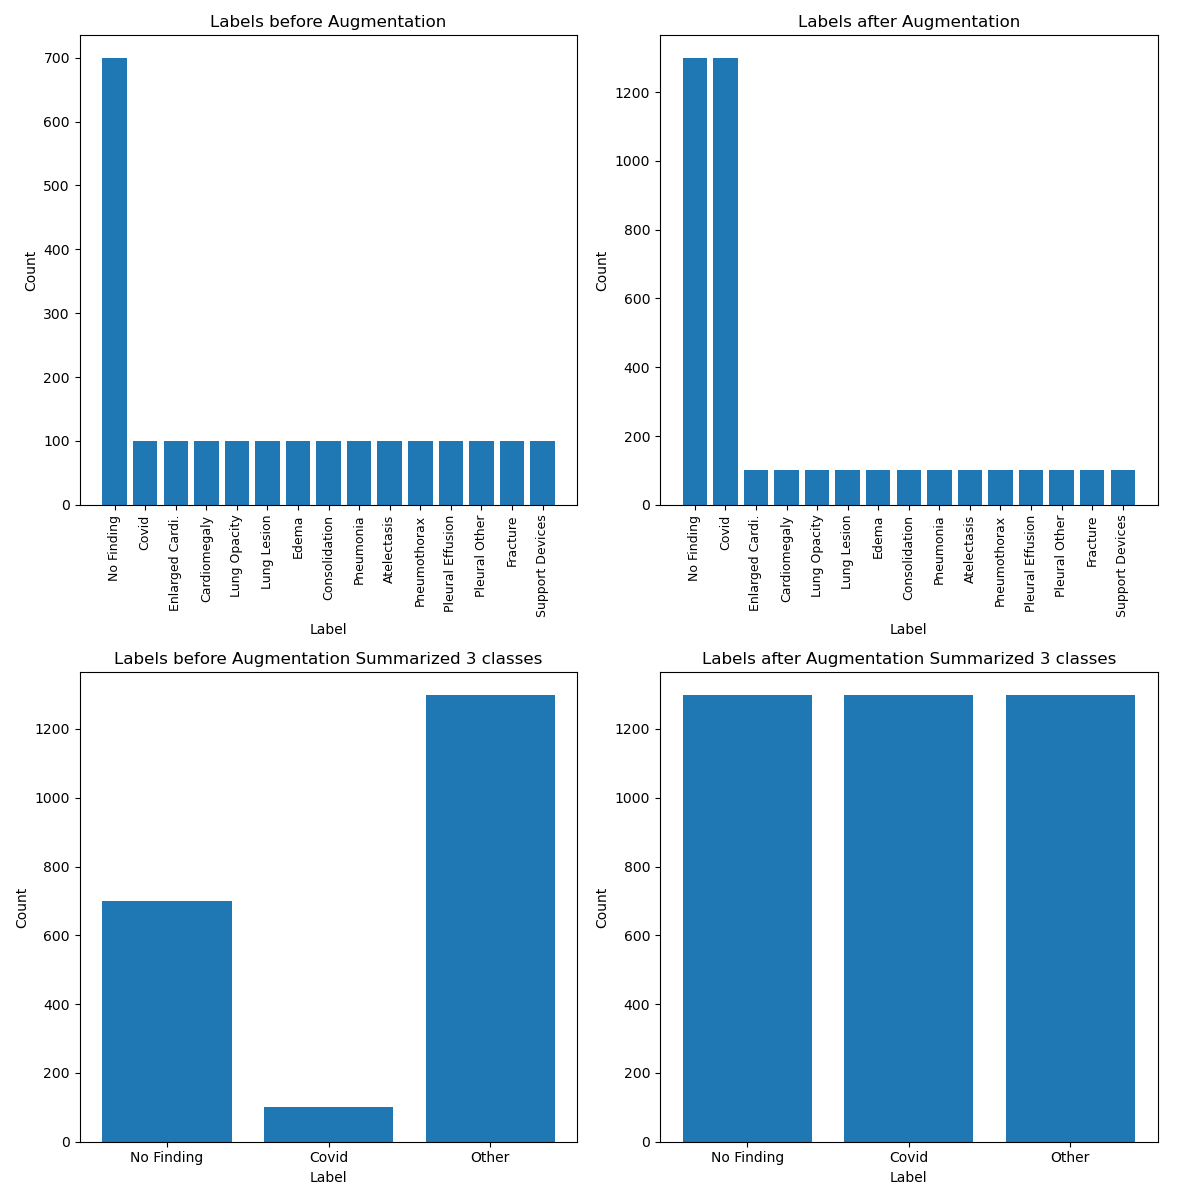
\includegraphics{../results/balancing.png}}
	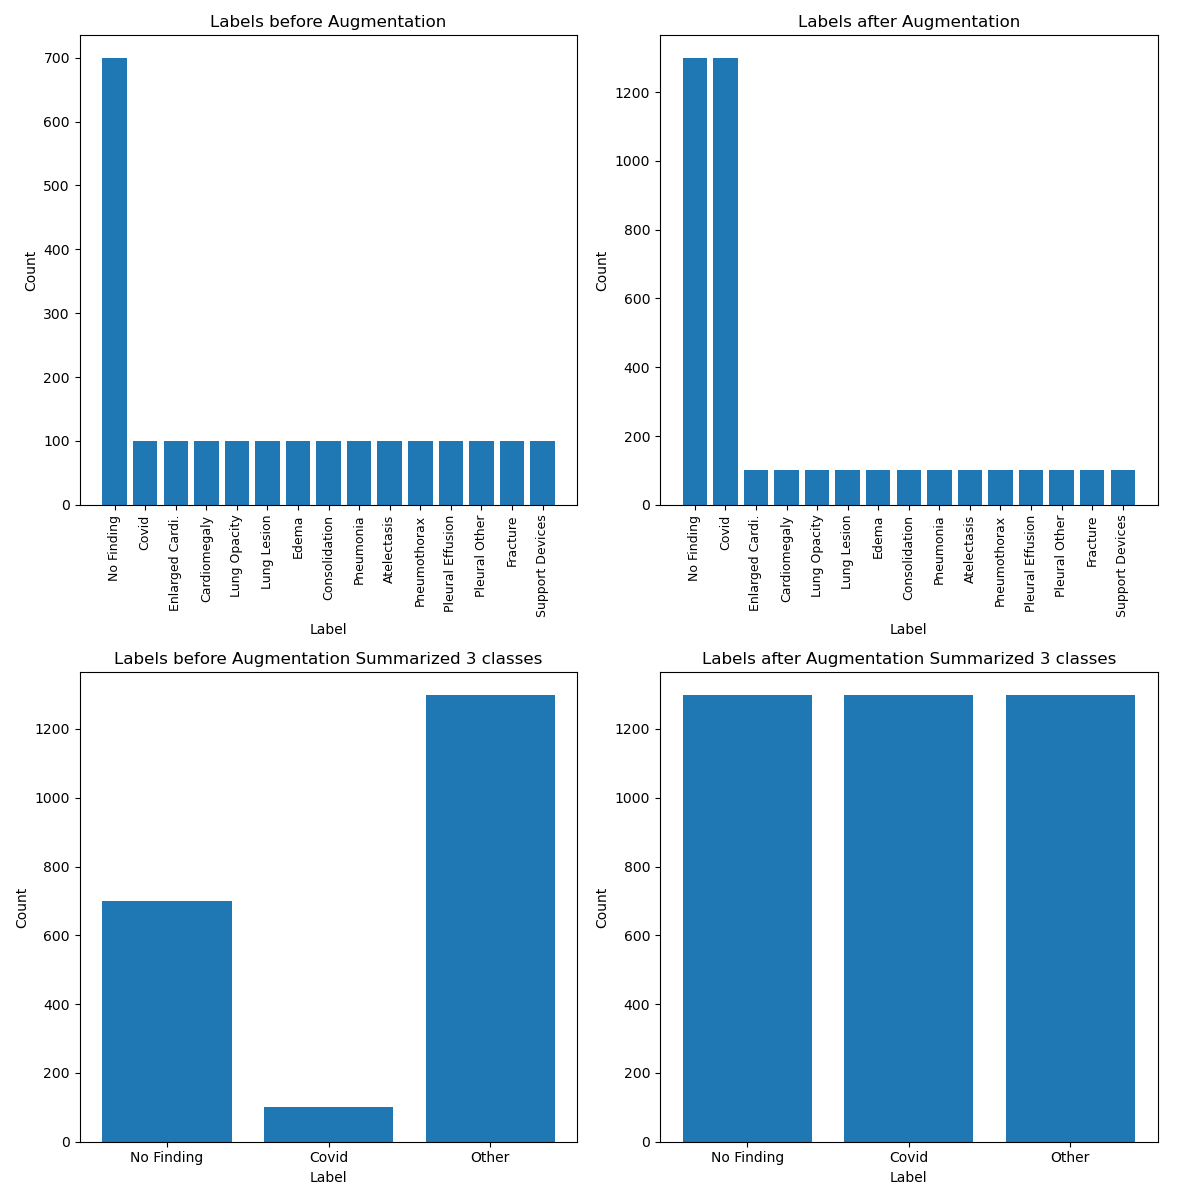
\includegraphics[trim=0.5\imagewidth{} 0 0 0, clip,width=0.3\imagewidth{}]{../results/balancing.png}
	\caption{Verteilung der Klassen nach Datenaugmentation}
	\label{fig:balancing}
\end{figure}

\section{Implementierung}

Zur Vorverarbeitung der Bilddaten und der Datenaugmentation dient das Python-Script \verb|preprocess.py|.

\begin{verbatim}
python preprocessing/preprocess.py [-h] [dataset] [output] [figure_output]
\end{verbatim}

Das \verb|dataset| Argument gibt analog zu den anderen Scripten das Verzeichnis an unter dem das Datenset zu finden ist. Zusätzlich können über \verb|output| und \verb|figure_output| die Ausgabeverzeichnisse für die erzeugten Bilder und Grafiken bestimmt werden.\\
Es steht eine Programmhilfe über den Parameter \verb|-h| zur Verfügung.
